%%% TOTO JE ORIGINÁLNA VERZIA SÚBORU, HLAVNÝ SÚBOR JE MAINCLANOK.TEX

% !TEX TS-program = pdflatex
% !TEX encoding = UTF-8 Unicode

\documentclass[11pt]{article}

\usepackage[utf8]{inputenc}
\usepackage{amsmath}

%LANGUAGE
\usepackage[T1]{fontenc}
\usepackage[utf8]{inputenc}   % UTF-8
\usepackage[slovak]{babel}    % pre slovenský jazyk

%DIMENZIE
\usepackage{geometry}
\geometry{a4paper}
\usepackage{geometry}
\geometry{
    a4paper,
    top=2.5cm,      % Pole hore
    bottom=2cm,     % Pole dole
    left=3cm,       % Ľavé pole
    right=1.5cm,    % Prave pole
    headheight=14pt % Výška colontitula 
}

\usepackage{graphicx} 
\usepackage[IL2]{fontenc}
%PACKAGES
\usepackage{booktabs} 
\usepackage{array} 
\usepackage{paralist} 
\usepackage{verbatim} 
\usepackage{subfig} 

% HEADERS & FOOTERS
\usepackage{fancyhdr}
\pagestyle{fancy} 
\renewcommand{\headrulewidth}{0pt}
\lhead{}\chead{}\rhead{}
\lfoot{}\cfoot{\thepage}\rfoot{}

\usepackage{sectsty}
\allsectionsfont{\sffamily\mdseries\upshape}

\usepackage[nottoc,notlof,notlot]{tocbibind} 
\usepackage[titles,subfigure]{tocloft} 
\renewcommand{\cftsecfont}{\rmfamily\mdseries\upshape}
\renewcommand{\cftsecpagefont}{\rmfamily\mdseries\upshape}

\title{ \bf Výskum WiFi HaLow Technológie}
\author{Adam Kšenzulák\and Arsenii Leno\and Oleh Kysil\and Tobias Lačný}
\date{}

\begin{document}
\maketitle
\paragraph {\bf Akronym: \tt ReWiLow}
\section*{\bf Charakteristika projektu}

Naša skupina skúma štandard IEEE 802.11ah pre LPWAN (Low Power Wide Area Network – Nízkoenergetická rozsiahla sieť), bežne známy ako Wi-fi HaLow, so zameraním  na jeho architektonický dizajn, výkonové charakteristiky a vhodnosť pre komunikáciu v rámci Internetu vecí (IoT), komuníkaciu medzi strojmi (M2M) aj na trhu. Skúmané sú aj jedinečné technické vlastnosti HaLow, ako pre prevádzka pod 1GHz v nelicencovaných rádiových (ISM) pásiem, rozsšírený dosah, nízka spotreba energie, a aj vysoká hustota zariadení. Hodnotená je aj jeho použiteľnosť v reálnych scenároch, vrátane inteligentného poľnohospodárstva, priemyselnej automatizácie, monitorovania životného prostredia a inteligentných miest.
V rámci projektu sa bude zameriavať aj na komparatívnu analýzu medzi Wi-Fi HaLow a inými LPWAN technológiami, príkladom sú LoRaWAN, Sigfox, alebo aj NB IoT najmä v ich parametroch, ako sú dosah, rýchlosť prenosu dát, latencia, energetická účinnosť a škálovateľnosť siete. Našim cieľom bude určiť konkrétne kontexty, v ktorých Wi-Fi HaLow ponúka výhody alebo obmedzenia v porovnaní s konkurečnými riešeniami LPWAN. Výsledky majú slúžiť ako podklad pre budúci rozvoj infraštruktúry IoT a stratégií konektivity na Slovensku

\section*{\bf Všeobecne údaje}

% Druhý riadok (Nízkoprúdové rozsiahle siete (LPWAN)) bude upravený ako
% podnadpis/hlavný predmet v tučnom, väčšom písme (napr. \subsection*),
% čím získa lepšiu vizuálnu hierarchiu.

\subsection*{\bf Nízkoprúdové Rozsiahle Siete (LPWAN)}

\noindent
\textbf{Nízkoprúdová rozsiahla sieť} (Low-Power, Wide-Area Network – \textbf{LPWAN} alebo \textbf{LPWA}) predstavuje špecifický typ bezdrôtovej telekomunikačnej rozsiahlej siete. Jej primárnym účelom je umožniť \textbf{komunikáciu na dlhé vzdialenosti} pri \textbf{nízkej bitovej rýchlosti}. Táto architektúra je navrhnutá predovšetkým na pripojenie zariadení \textbf{internetu vecí (IoT)}, ako sú senzory, ktoré sú typicky napájané z batérie.

\vspace{0.5\baselineskip} % Malý vertikálny priestor medzi odsekmi

\noindent
Charakteristické vlastnosti, ako sú \textbf{nízka spotreba energie}, obmedzená prenosová rýchlosť a špecifické určenie použitia, odlišujú siete LPWAN od klasických bezdrôtových rozsiahlych sietí (\textbf{WWAN}). Klasické WWAN sú totiž optimalizované na pripojenie koncových používateľov alebo podnikov a sú dimenzované na prenos väčšieho objemu dát pri vyššej spotrebe energie. Dátová priepustnosť v sieťach LPWAN sa obvykle pohybuje v rozmedzí \textbf{od $0.3\ \text{kbit/s}$ do $50\ \text{kbit/s}$} na kanál.

\vspace{0.5\baselineskip}

\noindent
LPWAN technológie umožňujú vytvorenie \textbf{privátnych bezdrôtových senzorových sietí}. Zároveň môžu byť ponúkané ako \textbf{infraštruktúrna služba} tretej strany. Táto možnosť eliminuje pre majiteľov senzorov nutnosť investovať do vlastnej \textbf{gateway} (\textbf{bránovej}) technológie, čím sa zjednodušuje a urýchľuje nasadenie zariadení v teréne.

\subsection*{\bf Princíp fungovania LPWAN}

\noindent
Základom princípu prenosu dát technológiou LPWAN na fyzickej vrstve PHY je \textbf{vlastnosť rádiových systémov} – \textit{zvýšenie energie,} a tým aj dosahu komunikácie pri \textit{znížení prenosovej rýchlosti}. Čím \textbf{nižšia je prenosová bitová rýchlosť}, tým viac energie sa vkladá do každého bitu, a tým \textbf{ľahšie je ho rozlíšiť} na pozadí šumu v prijímacej časti systému. Nízka prenosová rýchlosť dát teda umožňuje dosiahnuť väčší dosah ich príjmu.

\vspace{0.5\baselineskip}

\noindent

Prístup používaný na konštrukciu LPWAN-siete je \textbf{podobný} princípu fungovania \textbf{mobilných komunikačných sietí}. LPWAN-sieť využíva topológiu \textit{„hviezda“}, kde každé zariadenie komunikuje priamo so základňovou stanicou. Mestské alebo regionálne siete sa konštrujujú s použitím konfigurácie „hviezda z hviezd“.

\begin{figure}
    \centering
    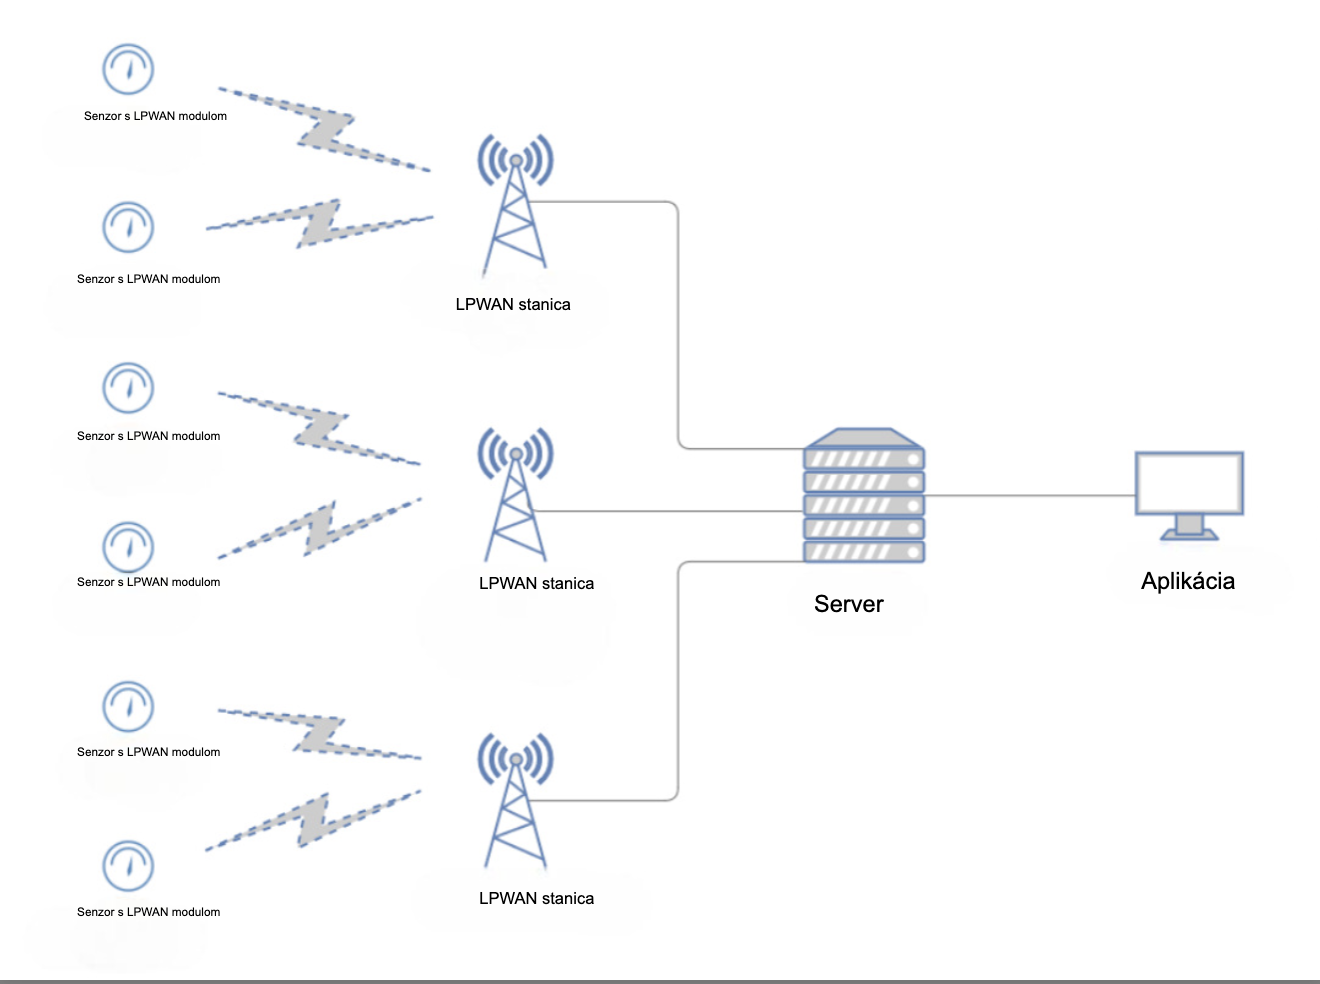
\includegraphics[width=0.5\linewidth]{LPWAN_pc1.png}
    \caption{LPWAN sieť}
    \label{fig:pc1}
\end{figure}

% 3. Pouzitie vo svete
\section*{\bf Použitie LPWAN }

\noindent
\subsection*{\bf Súčasné použitie technológie LPWAN vo svete}

\subsection*{\bf Perspektívy rozvoja a využitia LPWAN v budúcnosti}

\end{document}

\end{document}
